\section{Overview}\label{sec:overview}

In this section, we first describe \xxx event graphs
(\S\ref{subsec:eventgraph}). Then we explain how \xxx diagnoses performance
anomaly with a concrete example(\S\ref{subsec:overflow}).

\subsection{Event Graph Basics}\label{subsec:eventgraph}

The event graph is a generalized control-flow graph which includes inter-thread
and inter-process dependencies. To construct event graphs, \xxx collects three
categories of events in its systems-wide event logs. The first category of
events are boundary events that mark the beginning and ending of execution
segments. \xxx handles common callbacks, such as \vv{dispatch\_client\_callout}
and \vv{CFRunLoopDoBlocks}, and mark their entry and return as boundaries.
Every execution segment corresponds to a vertex in the event graph. The second
category contains semantic events, including system calls, call stacks when
certain operations such as \vv{mach\_msg} are running, and user actions such as
key presses. These events are stored as contents in the vertex and primarily for
providing information to user during diagnosis. The third category of events are
communication events for forming edges in the graph. For instance, an operation
that installs a callback is connected to the invocation of the callback. They
help users diagnose bugs across thread/process boundaries.

%A message send is connected to a message receive. The arming of a
%timer is connected to the processing of the timer callback. 

A unique design in \xxx is to trace general wake-up and wait operations inside
the kernel to ensure coverage across many diverse user-level, possibly custom
wake-up and wait operations because their implementations almost always use
kernel wake-up and wait. This approach necessarily includes spurious edges
in the graph, including those due to mutual exclusion and context switch by
interrupts; \xxx handles them by querying the user when it encounters a vertex
with multiple incoming causal edges during diagnosis (see \S\ref{subsec:overflow}).
We also observed that a waiting kernel thread is frequently woken up to perform
tasks such as timer firing signal and scheduler maintenance; \xxx recognizes
them and culls them out from the graph automatically.

Compared to tools such as \spindump that capture only the current system state,
event graphs capture the causal path of events, enabling users to trace across
threads and processes to events happened in the past (hence cannot be captured by
\spindump) that explain present anomalies. Therefore \xxx can report
root causes such as dead locks due to design flaws.

%% Given the prevalent of multi-threading and multi-processing programs, bugs are
%% much more complicated. The long opening bugs are usually have several threads
%% involve, even across process boundaries. As an example, the always timeout on
%% particular synchronization primitive in one thread usually need to trace back to
%% find the other thread that was responsible for signal the primitive. Compared
%% to the existing debugging tools like lldb and spindump, the dependency graph is
%% useful in that 1) it provides thread relationships all over the system across
%% process boundary and timing boundary and 2) it records execution history for an
%% input event before users capture hangs with their eyes.



\subsection{Argus Work Flow} \label{subsec:overflow}

\begin{figure}[tb]
    \centering
	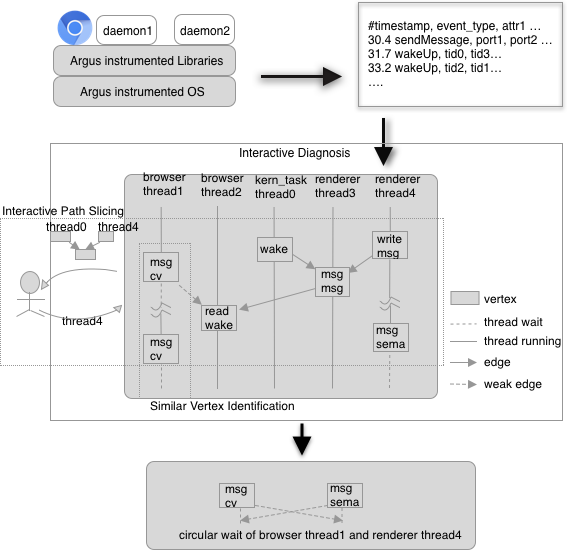
\includegraphics[width=\columnwidth]{./figures/Argus_overview.png}
    \caption{\xxx Work Flow}
    \label{fig:argus-overview}
\end{figure}

In this section, we describe the steps a tech-savvy user takes to investigate a
performance anomaly with \xxx.  Figure~\ref{fig:argus-overview} shows \xxx's
work flow with an example of a user investigating a performance problem in
Chromium.  The system wide tracing tool, which collects data from \xxx
instrumented library and kernel, generates logs. They are transformed into an
\emph{event graph} in \xxx's graph construction component. Diagnosis and
inference are performed within this graph, in a semi-automated fashion.  As
shown in Figure~\ref{fig:argus-overview}, the \xxx interactive debugger asks
the user to choose one edge in a subgraph. With this type of interaction, \xxx
runs its diagnosis algorithm and reports the root cause vertices.  Next, we
describe how \xxx assists the user to diagnose a performance issue.

\subsubsection{Initiate the diagnosis}

Compared to prior works which try to identify performance issue with critical
paths, \xxx takes the reported issue by system or users as input. It leverages
the semantic events in the graph to locate the vertex representing the reported
issue and initiate the diganosis.

Consider a common performance bug on macOS, the \emph{spinning cursor}, which
indicates the current application's main thread has not processed any UI events
for over two seconds. \vv{WindowServer} throws \vv{spinning cursor} with the
collaboration of the application's \vv{NSEvent} thread. The \vv{NSEvent}
thread fetches \vv{CoreGraphics} events from \vv{WindowServer}, converts and
creates \vv{NSApp} events for the main thread, and arms a timer to monitor
the event's wait time. If the main thread fails to process an event before
the timer fires, the \vv{NSEvent} thread notifies \vv{WindowServer} via
``\vv{CGSConnectionSetSpinning}'', and \vv{WindowServer} draws a \vv{spinning
cursor}.

To initialize debugging a \vv{spinning cursor}, \xxx first constructs an event
graph from the system-wide event log.  It then checks the semantic events from
the \vv{NSEvent} thread, identifies the time when the perfomance anomaly
happens, the invocation of ``\vv{CGSConnectionSetSpinning}'', and finds
\spinningnode in the main thread which contains the ongoing events concurrent.

\subsubsection{Diagnosis with Graph}\label{subsec:debug}

\begin{algorithm}[ht!]
    \caption{Diagnosis algorithm.}
    \label{alg:alg-diagnosis}
\begin{algorithmic}[1]
\Require{g - EventGraph; spinning\_node - the node in the UI thread when the spinning cursor occurs}
\Ensure{node\_vector - root cause node or the sliced path}
\Statex
\Function{Diagnose}{EventGraph g, Node *spinning\_node}
  \Switch {spinning\_node.block\_type}
    \Case {CPUBusy}
		\State {slice $\gets$ InteractiveSlice(spinning\_node)}
		\State\Return {slice}
	\EndCase
	\Case {Yield}
		\If {spinning\_node.NotContain(Share\_flag\_read\_Event)}
			\LineComment {Require users to annotate data flag}
			\State {abort()}
		\EndIf
		\LineComment {Fall through}
	\EndCase
	\Case {Wait}
		\LineComment {Find a baseline case where the wakeup occured}
		\State {normal\_nodes $\gets$ FindSimilar(spinning\_node)}
		\State {normal\_node $\gets$ Users.Pick(normal\_nodes)}
		\State {slice $\gets$ InteractiveSlice(normal\_node)} 	
		\State {$T_{spinning}$ $\gets$ spinning\_node.begin\_time}

		\For {$node$ $\gets$ $slice.begin().next()$ to $slice.end()$}
			\State {$T_{normal}$ $\gets$ node.end\_time}
			\State {$t$ $\gets$ node.thread}
			\State {$t\_nodes$ $\gets$ GetNodes(t, $T_{normal}$, $T_{spinning}$)}
			\For {$node_i$ $\gets$ $t\_nodes.begin()$ to $t\_nodes.end()$}
				\If {$node_i$.EventType == Wait}
					\State {node\_vector.append($node_i$)}
					\LineComment {Ask user if it is the root cause}
					\If {User.Yes}
						\State\Return {node\_vector}
					\Else
						\State {Diagnose($node_i$)}
					\EndIf
				\EndIf
			\EndFor
		\EndFor
		\LineComment {Fail to diagnose with blocking culprit, return the normal}
		\LineComment {node's parent for user to apply concrete debugging}
		\If {node\_vector.empty()}
			\State\Return {normal\_node.parent()}
		\EndIf
	\EndCase
  \EndSwitch
\EndFunction
\end{algorithmic}
\end{algorithm}


\begin{algorithm}[ht!]
    \caption{InteractiveSlicing algorithm.}
    \label{alg:alg-interactiveslicing}
\begin{algorithmic}[1]
\Require{g - EventGraph; node - the node user wants to slice from}
\Ensure{slice - causual path for node}
\Statex
\Function{InteractiveSlicing}{EventGraph g, Node *node}
\Loop
	\State{slice.append(node)}
	\If{node.parent().size() > 1}
		\State{node $\gets$ User.pick(candidates)}
		\If{node.NotExist()}
			\State\Return {slice}
		\EndIf
	\ElsIf{node.parent().size() == 1}
		\State{node $\gets$ node.parent().front()}
	\ElsIf{node.WeakEdges().size() > 0}
		\State{node $\gets$ User.Pick(weak edges)}
		\If{node.NotExist()}
			\State\Return {slice}
		\EndIf
	\Else
		\State\Return {slice}
	\EndIf
\EndLoop
\EndFunction
\end{algorithmic}
\end{algorithm}


Given the event graph and the \spinningnode, \xxx runs
Algorithm~\ref{alg:alg-diagnosis} to pinpoint the root cause.  Specifically,
upon examining what the main thread is actually doing, there are three
potential cases.

\begin{itemize}
	\item \textbf{LongRunning} (lines~\ref{a1:longrunning_begin}
		-~\ref{a1:longrunning_end}). The main thread is busy performing lengthy
		CPU operations. This case is the simplest, and \xxx traverses the event
		graph backwards to find a slice originating from the offending UI event
		to the long running CPU operations. This slice is particularly useful for
		further diagnosing the bug. As shown in Function \textit{InteractiveSlice} in
		line~\ref{alg:interslice-line}, \xxx may encounter vertices with multiple
		incoming edges or weak edges that do not reflect causality when traversing
		the graph. It queries the user to resolve them.

	\item \textbf{RepeatedYield} (lines~\ref{a1:repeatedyield_begin}
		-~\ref{a1:repeatedyield_end}). The main thread is in a yield loop, which
		is highly indicative it is waiting on a data flag (\eg, ``while(!done)
		thread\_switch();''). If \xxx cannot find any record of data flags in the
		\spinningnode, it terminates debugging by prompting the user to identify data
		flags and re-trace the application. Here we assume that the performance issue
		reproduces with a reasonable probability because, fortunately, a one-off issue
		that never reproduces is not as annoying as one that occurs frequently. If
		\xxx finds the data flag the \spinningnode is waiting for, it falls through to
		the next case.

	\item \textbf{LongWait} (lines~\ref{a1:longwait_begin}
		-~\ref{a1:longwait_end}). The main thread is in a lengthy blocking wait and
		the wake-up has been missing. \xxx handles this case by finding a normal
		scenario where the wake-up indeed arrives, and then figures out which wake-up
		edge is missing in the spinning scenario along the expected wake-up path.
		Specifically, \xxx first finds a \similarnode to the spinning one based
		on the event sequences in each vertex(\ref{subsec:similarvertex}). It then traverses
		backwards from the \similarnode to find the normal wake-up path. For each
		thread in the wake-up path, it examines the vertex in the thread right before
		the \spinningnode waits. If this vertex is also abnormal, \xxx appends it
		to the path of \rootcausenodes, and applies Function \textit{Diagnose} recursively
		to diagnose ``the culprit of the culprit''. For each such vertex, it queries the
		user to determine whether to proceed or stop, because based on our experience
		a few iterations are adequate to manifest the root cause.
		%the user needs to inspect only a few vertices to find the root cause.

\end{itemize}
\noindent
Our experience suggests that the first case is the most common, but the
second and third represent more severe bugs. Long-running CPU operations tend to
be more straightforward to diagnose with existing tools such as \spindump except
they do not connect CPU operations back to daemons and UI events. Repeated yielding or
long waiting cases involve multiple threads and processes, and are extremely
hard to understand and fix even for the application's original developers.
Therefore, issues remain unaddressed for years and significantly impact the
user experience. Algorithm~\ref{alg:alg-diagnosis} is semi-automated but can
integrate user input to leverage hypotheses or expert knowledge
as to why a hang may occur. Our results show that user inputs, albeit few, are
crucial in this process (\S\ref{sec:casestudy}).

\subsubsection{Chromium Spinning Cursor Example}

\begin{figure}[tb]
	\footnotesize
    \centering
	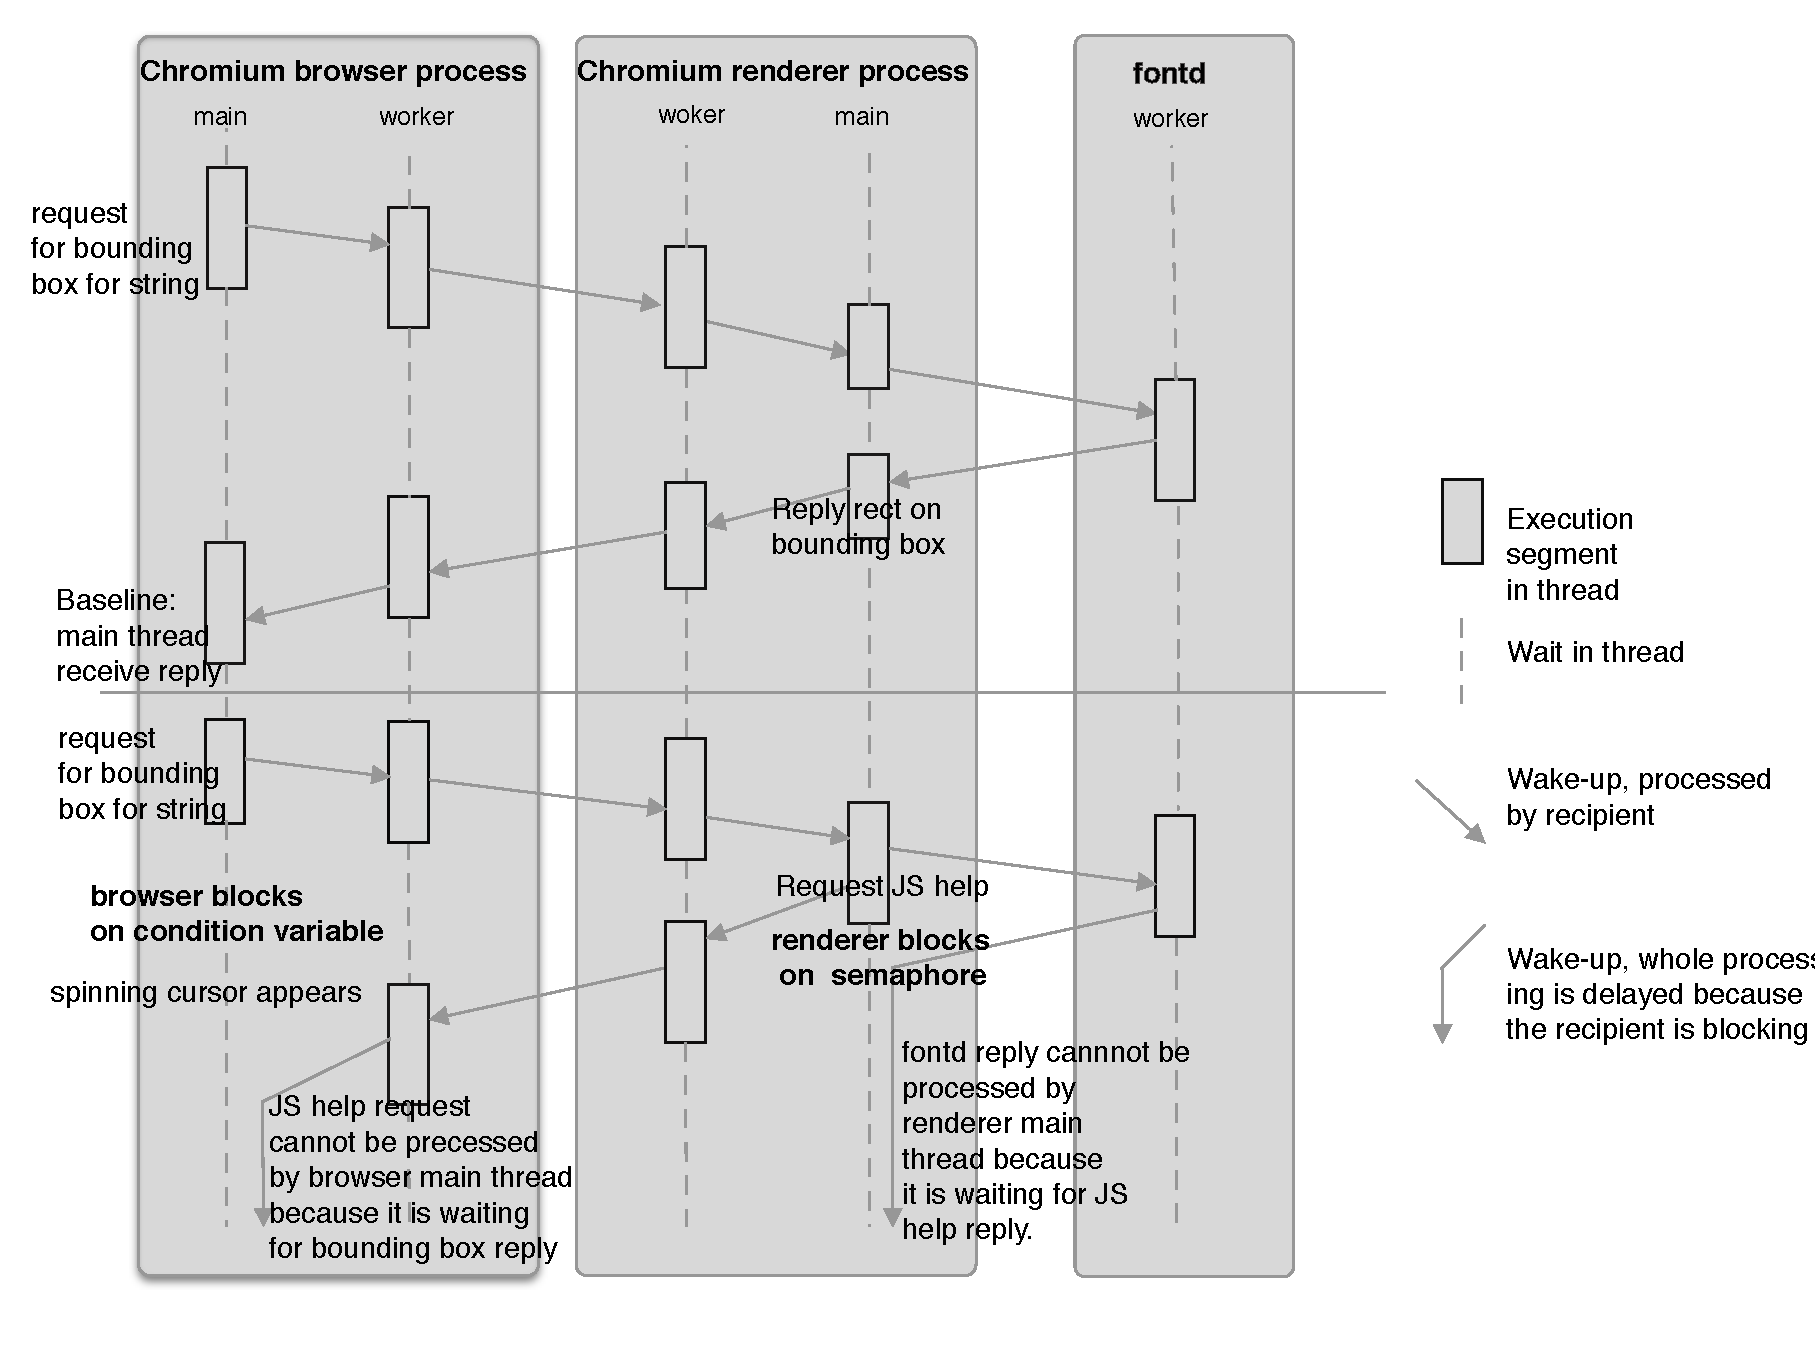
\includegraphics[width=\columnwidth]{./figures/chromium_case_study_2.pdf}
    \caption{Chromium Spinning Cursor Example}
    \label{fig:chromium-case-study}
\end{figure}

One of the authors experienced first-hand the aforementioned performance issue
in Chromium, an open-source browser engine that powers Google Chrome and,
starting recently, Microsoft Edge~\cite{chromiumurl}. She tried to type in
the Chromium search box a non-English word with a default Input Method Editor
shipped with MacOS. The browser appeared frozen and the spinning cursor showed
for a few seconds. Afterwards everything went back to normal. This issue is
reproducible and always ruins her experience, but is quite challenging to
diagnose because two applications Chromium and IME and many daemons ran and
exchanged messages. It was reported by other users for other non-English input
methods, too.

To diagnose this issue with \xxx, the author follows the steps in
Figure~\ref{fig:argus-overview}. She started system-wide tracing, and then
reproduced the spinning cursor with a non-English search string while the
page was loading. After the very first few characters which the browser
handles normally, the remaining characters triggered a spinning cursor. The
entire session took roughly five minutes. She then ran \xxx to construct
the event graph. The graph was highly complex, with 2,749,628 vertices and
3,606,657 edges, almost fully connected. It spanned across 17 applications;
109 daemons including \vv{fontd}, \vv{mdworker}, \vv{nsurlsessiond} and
helper tools by applications; 126 processes; 679 threads, and 829,287
messages. Given the scale of the graph and the diverse communication patterns,
it would be extremely challenging for prior automated causal tracing
tools~\cite{aguilera2003performance, zhang2013panappticon, attariyan2012x,
cohen2004correlating} because they handle a limited set of patterns. Tools
that require manual schema~\cite{barham2004using, reynolds2006pip}, would be
prohibitive because developers would have to provide schema for all involved
applications and daemons.

Next she ran \xxx to find the \spinningnode in the main thread of the browser
process. \xxx returned a \vv{LongWait} event, a \vv{psynch\_cv\_wait()} with a
timeout of 1.5 seconds, and identified a \similarnode in normal scenario where
the \vv{wait} was signaled quickly.

\xxx then found the normal wake-up path with interactive path slicing,
which connects five threads. The \vv{browser} main thread was signaled
by a \vv{browser} worker thread, which received IPC from a worker thread
of \vv{renderer} where the rendering view and WebKit code run. This
worker thread is woken up by the \vv{renderer} main thread, which in
turn woken by \vv{fontd}, the font service daemon, as shown in the upper
side of Figure~\ref{fig:chromium-case-study}. \xxx further compared
the normal case with the spinning case thread by thread as shown in
Figure~\ref{fig:chromium-case-study}, and returned the \vv{LongWait} event on
semaphore in the \vv{renderer} main thread, the culprit that delayed waking up
the \vv{browser} main thread over four seconds. What caused the wait in the
\vv{renderer} main thread though? She thus continued diagnosis and recursively
applied \xxx to the wait in \vv{renderer}(corresponding normal path is not shown
in the figure), and it turned out that \vv{renderer} was actually waiting for
the \vv{browser} main thread -- a circular wait formed.

Inspect of the reported vertices reveals that the \vv{browser} was waiting
for the \vv{renderer} to return the string bounding box for a string, and the
\vv{renderer} was waiting for the \vv{browser} to help render JavaScript.
This circular wait was broken by a timeout in the browser main thread (the
\vv{wait} on \vv{psynch\_cv\_wait()} timeouts in 1,500 ms). While the system
was able to make progress, the next key press caused the spinning cursor to
display for another 1,500 ms. The timeout essentially converted a deadlock
into a livelock. To verify this diagnosis, we shortened the timeout in the
\vv{psynch\_cv\_wait()} called in the Chromium browser to 150 ms, which
proportionally reduced how often this spinning cursor occurs.

\subsection{Similar Vertex Indetification}\label{subsec:similarvertex}

\xxx leverages a normal scenario to discover missing wake-up edges in \vv{LongWait}
cases. The normal scenario is identified from the \similarnode which shares
the same high level semantics as the \spinningnode, but exposes different
execution results.

\xxx identifies the \similarnodes first by inferring its high level semantics
with semantic events, and its programming purpose with communication events
which form edges in the graph. The semantic events include system calls, call
stacks, and user inputs. Their sequential order and runtime unrelated attributes
are treated as hallmarks. For example, in call stacks, \xxx compares vertices
with symbol names instead of memory addresses. The communication events include
messages, dispatch queue operations, runloop operations, \dataflagread and
\dataflagwrite. The process names of peer vertices are checked, as they reflect
the developers' intent, for example, to request service from a particular
helper tool. More over, a user can also instruct \xxx to inspect preceeding
vertices to improve identification accuracy. Then \xxx discriminate the
execution results to filter out spinning scenarios.  with the time cost and
wait result in the vertex by default. If multiple \similarnodes are identified,
\xxx usually chooses the most recent one heuristically.

\subsection{Limitations}

\xxx is designed to support interactive debugging of performance issues. It
sometimes requires the user to reproduce a performance issue so \xxx can capture
more fine-grained event traces such as accesses to data flags. Fortunately, a
performance issue that almost never reproduces is probably not as annoying as
one that occurs frequently.

We implemented \xxx in the closed-source macOS which presents a harsh test
for \xxx, but we have not ported \xxx to other operating systems yet. It is
possible that the ideas and techniques do not generalize to other operating
systems. However, modern operating systems share many similarities, and inspire
each others' designs, so we are hopeful that the ideas in \xxx are generally applicable.
Similarly, the applications and performance issues used in our
evaluation may be non-representative, though we strive to cover a diverse set of
common applications ranging from browsers to text editors.
